%!TEX root = ../dissertation.tex

\chapter{Tests and Results} \label{cha:test}

\section{Assembling Objects Test}\label{sec:ass_objs_test}

The torque reaction arm is ergonomic solution, basically a mechanical device, developed to absorb the reaction torque generated by the associated industrial tools, such as electronic and electric screwdrivers.
Torque reaction arms protect the operator from vibrations and reaction torques, improving safety in the workplace and preventing musculoskeletal disorders. \\

There are different types of arms, the assembly proposed here will compose a part of an BNP orthogonal torque reaction arms (BRF series, Figure \ref{fig:brf}). \\
Orthogonal torque reaction arms can be installed on the workbench thanks to the vertical sliding column that allows the arm to rotate around its axis. 
This arm allow orthogonal tightening operations to be performed to workbench plane. \\

\begin{figure} [h]
\centering
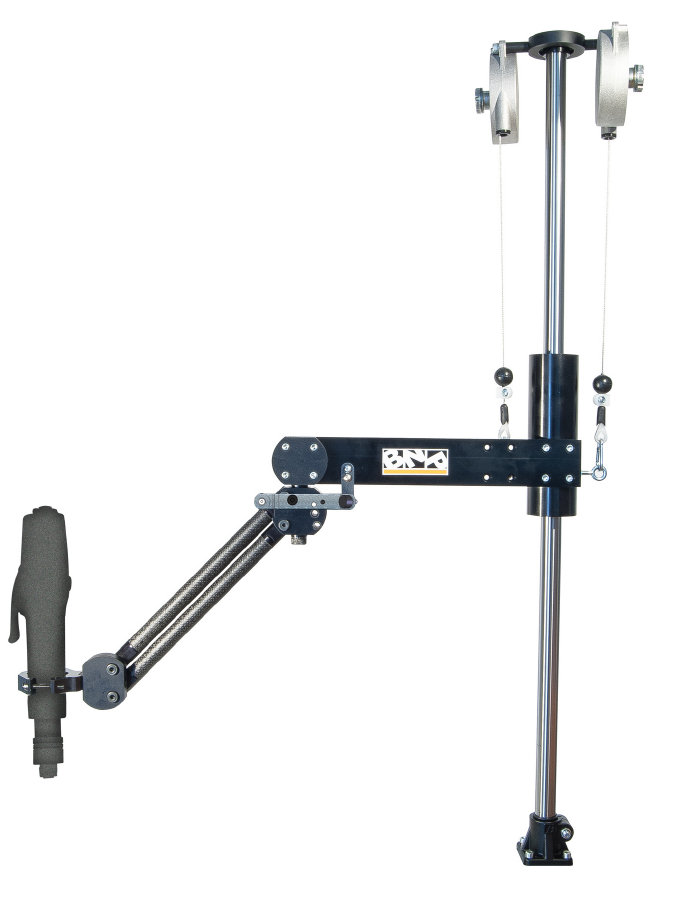
\includegraphics[width=0.6
\textwidth]{figures/Magistrale/BRF}
\caption[BNP Orthogonal Torque Reaction Arms]{BNP orthogonal torque reaction arms, BRF series. Folded arm which allows orthogonal tightening to workbench plane.
\label{fig:brf}}
\end{figure} 

The Table \ref{tab:ass_table} summarises the characteristics of the components that will be used: the Number, which is used in the figures below to indicate the component, the Quantity, the Colour Cube, which associates each component with a colour of the respective cube representing it (to better understand the simulation figures), Semantic Name, which is the name given to each component and which is used in the AtomSpace. \\

\begin{table}[htbp]
  \centering
  \caption{Assemblable Objects Description Table}\label{tab:ass_table}
  \medskip
\renewcommand\arraystretch{1.5}
\renewcommand\tabcolsep{12pt}
\begin{tabular}{cccc}
\toprule
\multicolumn{4}{c}{\textbf{Assemblable Objects}} \\
\textbf{Number} &  \textbf{Quantity} &  \textbf{Colour Cube} &  \textbf{Semantic Name}  \\
\midrule
\rowcolor{gray!25}
5 & 2 & Green / Orange & BearingSleeve1 / BearingSleeve2 \\
6 & 1 & Blue & BettClamp \\
\rowcolor{gray!25}
7 & 1 & - & Bearing \\
9 & 2 & Grey / Gold & SnapRing1 / SnapRing2 \\
\rowcolor{gray!25}
14 & 1 & - & TCEIScrew \\
31 & 1 & - & RotatingBalancerSupport \\
\rowcolor{gray!25}
32 & 1 & Red & RecirculatingBallSleeve \\
39 & 1 & - & UpperBearingBracket \\
\rowcolor{gray!25}
43 & 1 & Yellow & InductionHardenedRod \\
\bottomrule
\end{tabular}
\renewcommand\arraystretch{1}
\renewcommand\tabcolsep{5pt}
\end{table}

The arm assembly is schematically shown in Figure \ref{fig:brf_draw}. It is divided into three sub-assemblies:

\begin{enumerate}
	\item BlockA: the Bett clamp and the induction hardened rod are taken from their respective bins and mounted on top of the workbench (Figure \ref{fig:ass_obj_1}). Next, the resulting component will be called BlockA and will be represented by a single cube. Finally, it will be moved from the workbench to the table. \\

\begin{table}[htbp]
  \centering
  \caption{BlockA Assembly Process}\label{tab:ass_A_1}
  \medskip
\begin{tabular}{ll}
\toprule
\textbf{Parameters} &  \textbf{Values}  \\
\midrule
\rowcolor{gray!25}
Objects List &  InductionHardenedRod, BettClamp, SnapRing1, SnapRing2, \\
\rowcolor{gray!25}
& RecirculatingBallSleeve, BearingSleeve1, BearingSleeve2, table, \\
\rowcolor{gray!25}
& workbench, PurpleBin, GreenBin, RedBin, BlueBin, YellowBin \\
Additional Info. & The table is a fixed object. \\
& The workbench is a fixed object. \\
& The PurpleBin is a fixed object. \\
& The GreenBin is a fixed object. \\
& The RedBin is a fixed object. \\
& The BlueBin is a fixed object. \\
& The YellowBin is a fixed object. \\
\rowcolor{gray!25}
Request & The BettClamp is on the workbench. \\
\rowcolor{gray!25}
& The InductionHardenedRod is on the BettClamp. \\
Solution & (pickup (ConceptNode "BettClamp")) \\
& (stack (ConceptNode "BettClamp") (ConceptNode "workbench")) \\
& (pickup (ConceptNode "InductionHardenedRod")) \\
& (stack (ConceptNode "InductionHardenedRod") (ConceptNode "BettClamp")) \\
\rowcolor{gray!25}
Exec. Time & 25 sec \\
No. Iters. & 401 \\	
\bottomrule
\end{tabular}
\end{table}

\begin{table}[htbp]
  \centering
  \caption{BlockA Move Process}\label{tab:ass_A_2}
  \medskip
\begin{tabular}{ll}
\toprule
\textbf{Parameters} &  \textbf{Values}  \\
\midrule
\rowcolor{gray!25}
Objects List &  BlockA, SnapRing1, SnapRing2, RecirculatingBallSleeve, \\
\rowcolor{gray!25}
& BearingSleeve1, BearingSleeve2, table, workbench, \\
\rowcolor{gray!25}
&  PurpleBin, GreenBin, RedBin, BlueBin, YellowBin \\
Additional Info. & *** \\
\rowcolor{gray!25}
Request & The BlockA is on the table. \\
Solution & (pickup (ConceptNode "BlockA")) \\
& (stack (ConceptNode "BlockA") (ConceptNode "table")) \\
\rowcolor{gray!25}
Exec. Time & 0 sec \\
No. Iters. & 3 \\	
\bottomrule
\end{tabular}
\end{table}

	\item BlockB: Once the workbench is freed, the second piece is assembled, using 2 snap rings, 2 bearing sleeves and 1 recirculating ball sleeve (Figure \ref{fig:ass_obj_2}). It will be called BlockB and will then be inserted into BlockA (\textit{Stack BlockA BlockB}) on top of the table.

\begin{table}[htbp]
  \centering
  \caption{BlockB Assembly Process 1}\label{tab:ass_B_1}
  \medskip
\begin{tabular}{ll}
\toprule
\textbf{Parameters} &  \textbf{Values}  \\
\midrule
\rowcolor{gray!25}
Objects List &  BlockA, SnapRing1, SnapRing2, RecirculatingBallSleeve, \\
\rowcolor{gray!25}
& BearingSleeve1, BearingSleeve2, table, workbench, \\
\rowcolor{gray!25}
&  PurpleBin, GreenBin, RedBin, BlueBin, YellowBin \\
Additional Info. & *** \\
& The SnapRing1 is on the SnapRing2. \\
& The BearingSleeve1 is on the BearingSleeve2. \\
\rowcolor{gray!25}
Request & The SnapRing1 is on the workbench. \\
\rowcolor{gray!25}
& The BearingSleeve1 is on the SnapRing1. \\
Solution & (unstack (ConceptNode "SnapRing1") (ConceptNode "SnapRing2")) \\
& (stack (ConceptNode "SnapRing1") (ConceptNode "workbench")) \\
& (unstack (ConceptNode "BearingSleeve1")(ConceptNode "BearingSleeve2")) \\
& (stack (ConceptNode "BearingSleeve1") (ConceptNode "SnapRing1")) \\
\rowcolor{gray!25}
Exec. Time & 39 sec \\
No. Iters. & 493 \\	
\bottomrule
\end{tabular}
\end{table}

\begin{table}[htbp]
  \centering
  \caption{BlockB Assembly Process 2}\label{tab:ass_B_2}
  \medskip
\begin{tabular}{ll}
\toprule
\textbf{Parameters} &  \textbf{Values}  \\
\midrule
\rowcolor{gray!25}
Objects List &  BlockA, SnapRing1, SnapRing2, RecirculatingBallSleeve, \\
\rowcolor{gray!25}
& BearingSleeve1, BearingSleeve2, table, workbench, \\
\rowcolor{gray!25}
&  PurpleBin, GreenBin, RedBin, BlueBin, YellowBin \\
Additional Info. & *** \\
& The SnapRing1 is on the workbench. \\
& The BearingSleeve1 is on the SnapRing1. \\
& The RecirculatingBallSleeve is on the BearingSleeve1. \\
& The BearingSleeve2 is on the RecirculatingBallSleeve. \\
\rowcolor{gray!25}
Request & The SnapRing2 is on the BearingSleeve2. \\
Solution & (pickup (ConceptNode "RecirculatingBallSleeve")) \\
& (stack (ConceptNode "RecirculatingBallSleeve") (ConceptNode "BearingSleeve1")) \\
& (pickup (ConceptNode "BearingSleeve2")) \\
& (stack (ConceptNode "BearingSleeve2") (ConceptNode "RecirculatingBallSleeve")) \\
\rowcolor{gray!25}
Exec. Time & 21 sec \\
No. Iters. & 343 \\	
\bottomrule
\end{tabular}
\end{table}

\begin{table}[htbp]
  \centering
  \caption{BlockB Assembly Process 3}\label{tab:ass_B_3}
  \medskip
\begin{tabular}{ll}
\toprule
\textbf{Parameters} &  \textbf{Values}  \\
\midrule
\rowcolor{gray!25}
Objects List &  BlockA, SnapRing1, SnapRing2, RecirculatingBallSleeve, \\
\rowcolor{gray!25}
& BearingSleeve1, BearingSleeve2, table, workbench, \\
\rowcolor{gray!25}
&  PurpleBin, GreenBin, RedBin, BlueBin, YellowBin \\
Additional Info. & *** \\
& The SnapRing1 is on the workbench. \\
& The BearingSleeve1 is on the SnapRing1. \\
& The RecirculatingBallSleeve is on the BearingSleeve1. \\
& The BearingSleeve2 is on the RecirculatingBallSleeve. \\
\rowcolor{gray!25}
Request & The SnapRing2 is on the BearingSleeve2. \\
Solution & (pickup (ConceptNode "SnapRing2")) \\
& (stack (ConceptNode "SnapRing2") (ConceptNode "BearingSleeve2")) \\
\rowcolor{gray!25}
Exec. Time & 0 sec \\
No. Iters. & 3 \\	
\bottomrule
\end{tabular}
\end{table}

\begin{table}[htbp]
  \centering
  \caption{BlockB Move Process}\label{tab:ass_B_4}
  \medskip
\begin{tabular}{ll}
\toprule
\textbf{Parameters} &  \textbf{Values}  \\
\midrule
\rowcolor{gray!25}
Objects List &  BlockA, BlockB, table, workbench, \\
\rowcolor{gray!25}
&  PurpleBin, GreenBin, RedBin, BlueBin, YellowBin \\
Additional Info. & *** \\
\rowcolor{gray!25}
Request & The BlockB is on the BlockA. \\
Solution & (pickup (ConceptNode "BlockB")) \\
& (stack (ConceptNode "BlockB") (ConceptNode "BlockA")) \\
\rowcolor{gray!25}
Exec. Time & 0 sec \\
No. Iters. & 2 \\	
\bottomrule
\end{tabular}
\end{table}

	\item BlockC: Finally, the last piece, consisting of an upper bearing bracket, a bearing, a rotating balancer support and a TCEI screw, is mounted (Figure \ref{fig:ass_obj_2}). This will be BlockC and will be stacked on top of BlockB.
\end{enumerate}

\begin{table}[htbp]
  \centering
  \caption{BlockC Assembly Process 1}\label{tab:ass_C_1}
  \medskip
\begin{tabular}{ll}
\toprule
\textbf{Parameters} &  \textbf{Values}  \\
\midrule
\rowcolor{gray!25}
Objects List &  BlockA, BlockB, TCEIScrew, UpperBearingBracket, \\
\rowcolor{gray!25}
& RotatingBalancerSupport, Bearing, table, workbench, \\
\rowcolor{gray!25}
&  PurpleBin, GreenBin, RedBin, BlueBin, YellowBin \\
Additional Info. & *** \\
& The BlockB is on the BlockA. \\
\rowcolor{gray!25}
Request & The UpperBearingBracket is on the BlockC. \\
\rowcolor{gray!25}
& The Bearing is on the UpperBearingBracket. \\
\rowcolor{gray!25}
& The RotatingBalancerSupport is on the Bearing. \\
Solution & (pickup (ConceptNode "UpperBearingBracket")) \\
& (stack (ConceptNode "UpperBearingBracket") (ConceptNode "BlockC")) \\
& (pickup (ConceptNode "Bearing")) \\
& (stack (ConceptNode "Bearing") (ConceptNode "UpperBearingBracket")) \\
& (pickup (ConceptNode "RotatingBalancerSupport")) \\
& (stack (ConceptNode "RotatingBalancerSupport") (ConceptNode "Bearing")) \\
\rowcolor{gray!25}
Exec. Time & 699 sec \\
No. Iters. & 5853 \\	
\bottomrule
\end{tabular}
\end{table}

\begin{table}[htbp]
  \centering
  \caption{BlockC Assembly Process 2}\label{tab:ass_C_2}
  \medskip
\begin{tabular}{ll}
\toprule
\textbf{Parameters} &  \textbf{Values}  \\
\midrule
\rowcolor{gray!25}
Objects List &  BlockA, BlockB, TCEIScrew, UpperBearingBracket, \\
\rowcolor{gray!25}
& RotatingBalancerSupport, Bearing, table, workbench, \\
\rowcolor{gray!25}
&  PurpleBin, GreenBin, RedBin, BlueBin, YellowBin \\
Additional Info. & *** \\
& The BlockB is on the BlockA. \\
& The UpperBearingBracket is on the BlockC. \\
& The Bearing is on the UpperBearingBracket. \\
& The RotatingBalancerSupport is on the Bearing. \\
\rowcolor{gray!25}
Request & The TCEIScrew is on the RotatingBalancerSupport. \\
Solution & (pickup (ConceptNode "TCEIScrew")) \\
& (stack (ConceptNode "TCEIScrew") (ConceptNode "RotatingBalancerSupport")) \\
\rowcolor{gray!25}
Exec. Time & 0 sec \\
No. Iters. & 2 \\	
\bottomrule
\end{tabular}
\end{table}

\begin{table}[htbp]
  \centering
  \caption{BlockC Move Process}\label{tab:ass_C_3}
  \medskip
\begin{tabular}{ll}
\toprule
\textbf{Parameters} &  \textbf{Values}  \\
\midrule
\rowcolor{gray!25}
Objects List &  BlockA, BlockB, BlockC, table, workbench, \\
\rowcolor{gray!25}
&  PurpleBin, GreenBin, RedBin, BlueBin, YellowBin \\
Additional Info. & *** \\
& The BlockB is on the BlockA. \\
\rowcolor{gray!25}
Request & The BlockC is on the BlockB. \\
Solution & (pickup (ConceptNode "BlockC")) \\
& (stack (ConceptNode "BlockC") (ConceptNode "BlockB")) \\
\rowcolor{gray!25}
Exec. Time & 0 sec \\
No. Iters. & 3 \\	
\bottomrule
\end{tabular}
\end{table}

The Tables \ref{tab:ass_A_1}, \ref{tab:ass_A_2}
Tables \ref{tab:ass_B_1}, \ref{tab:ass_B_2}, \ref{tab:ass_B_3}, \ref{tab:ass_B_4}
Tables \ref{tab:ass_C_1}, \ref{tab:ass_C_2}, \ref{tab:ass_C_3}


\begin{figure} [h]
\centering
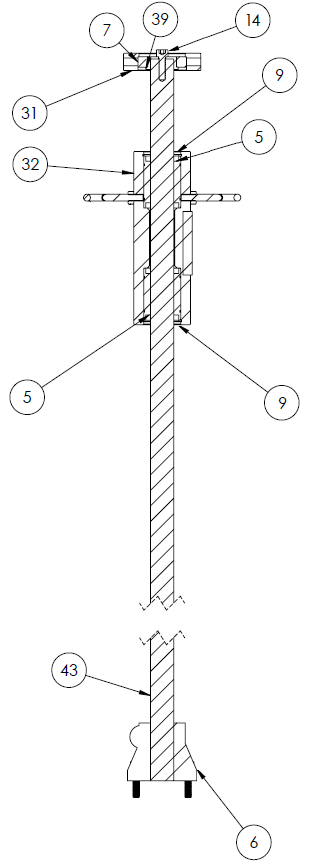
\includegraphics[width=0.25
\textwidth]{figures/Magistrale/BRF_draw}
\caption[Assembly Diagram]{
\label{fig:brf_draw}}
\end{figure} 

\begin{figure} [h]
\centering
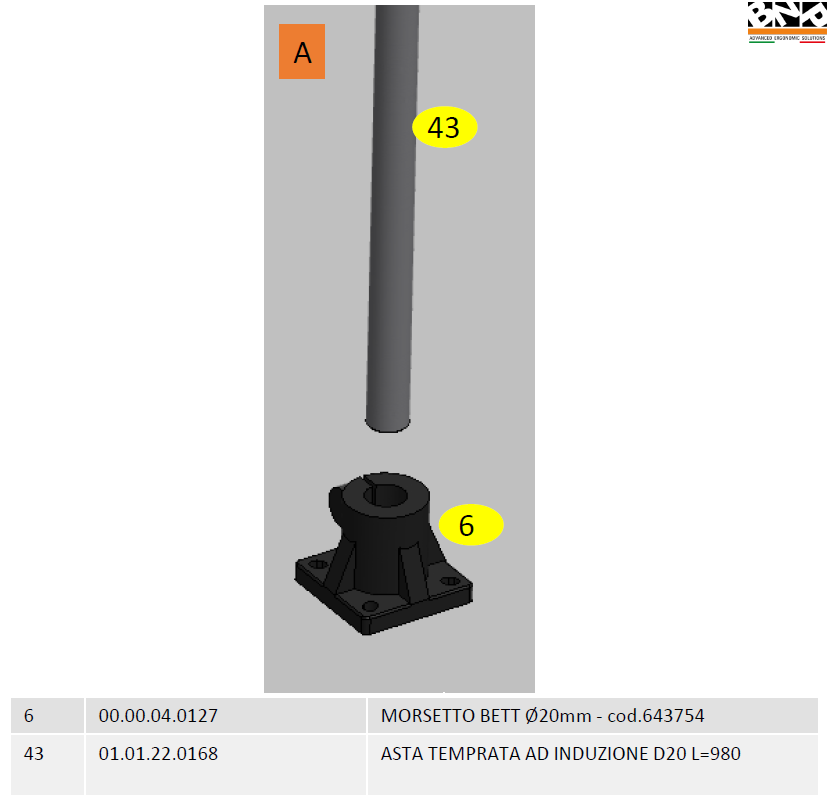
\includegraphics[width=0.6
\textwidth]{figures/Magistrale/ass_obj_1}
\caption[BlockA Assembly]{Assembly of BlockA
\label{fig:ass_obj_1}}
\end{figure} 

\begin{figure} [h]
\centering
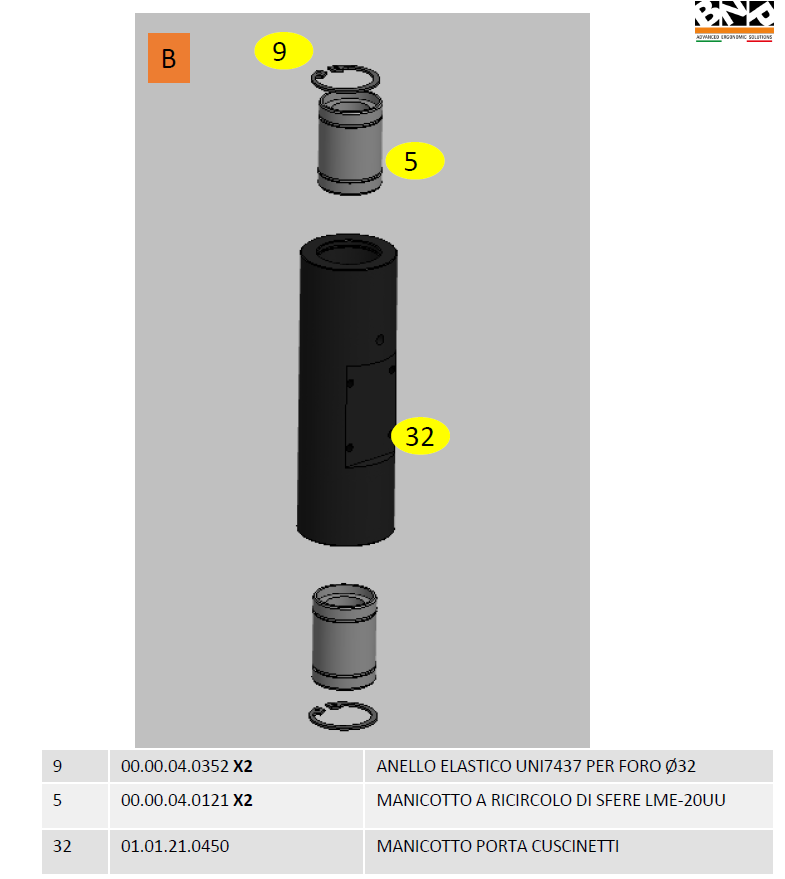
\includegraphics[width=0.6
\textwidth]{figures/Magistrale/ass_obj_2}
\caption[BlockB Assembly]{Assembly of BlockB
\label{fig:ass_obj_2}}
\end{figure} 

\begin{figure} [h]
\centering
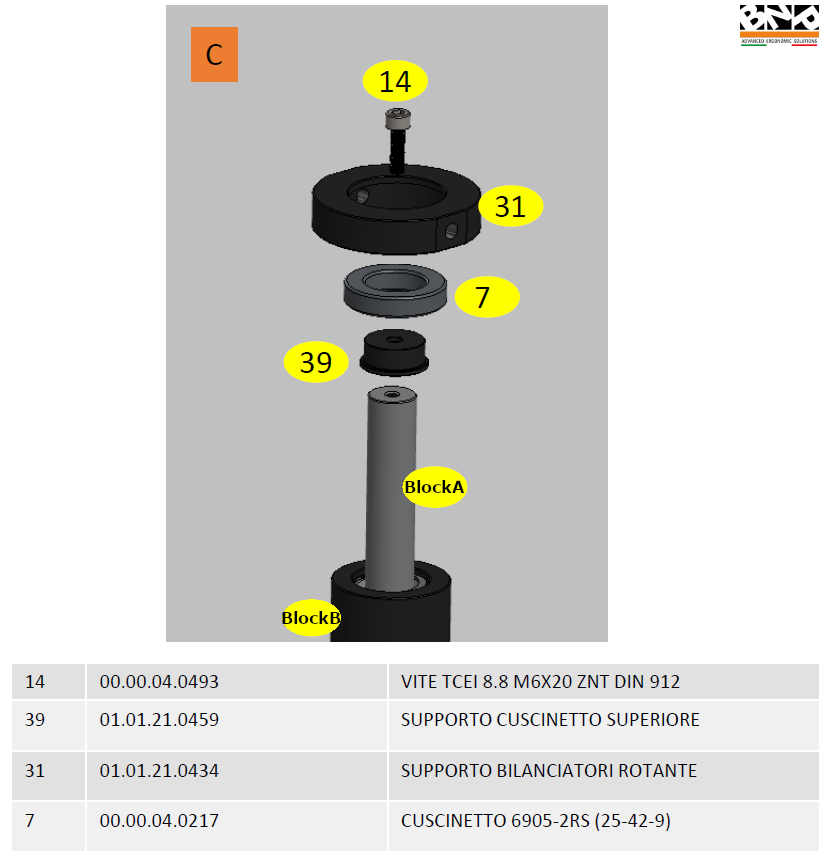
\includegraphics[width=0.6
\textwidth]{figures/Magistrale/ass_obj_3}
\caption[BlockC Assembly]{Assembly of BlockC
\label{fig:ass_obj_3}}
\end{figure} 

Assembly took place in a simulated environment, starting with the configuration shown in Figure \ref{fig:ass_1}.  Inside each bin. there are one or more cubes representing a component from the previous table. Components without Colour Cube (i.e. those in BlockC) are not shown in the simulation figures, both because BlockC is assembled in a similar way to BlockB, and to keep the illustrations clearer.


\begin{figure} [h]
\centering
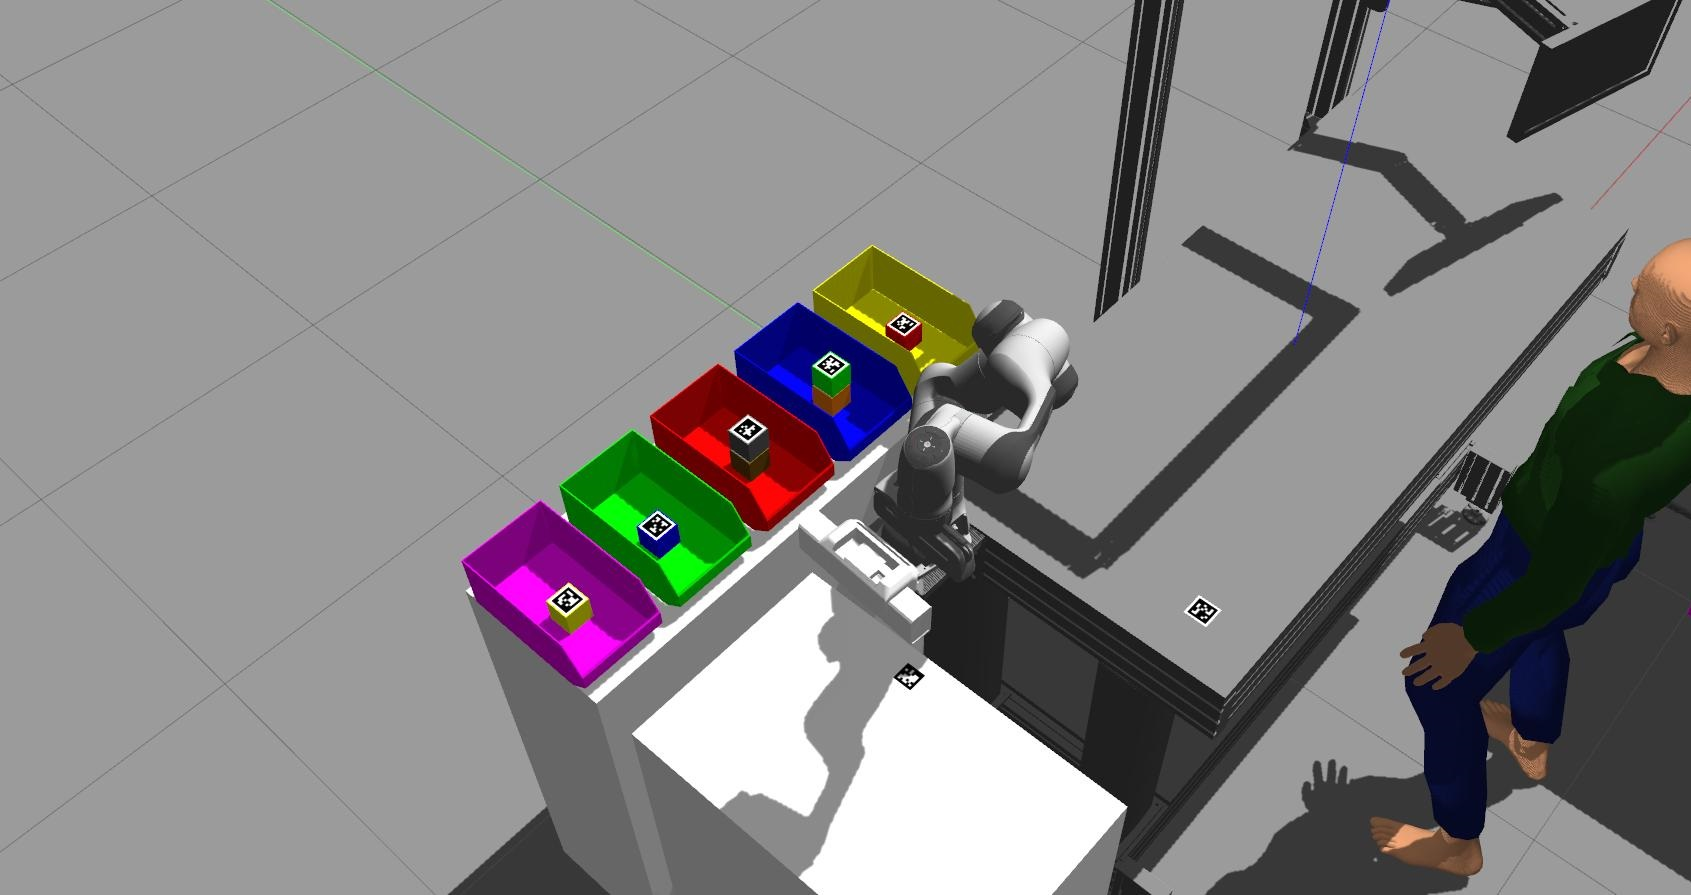
\includegraphics[width=0.6
\textwidth]{figures/Magistrale/ass_1}
\caption[Initial Assembly Test Environment]{
\label{fig:ass_1}}
\end{figure} 

\begin{figure} [h]
\centering
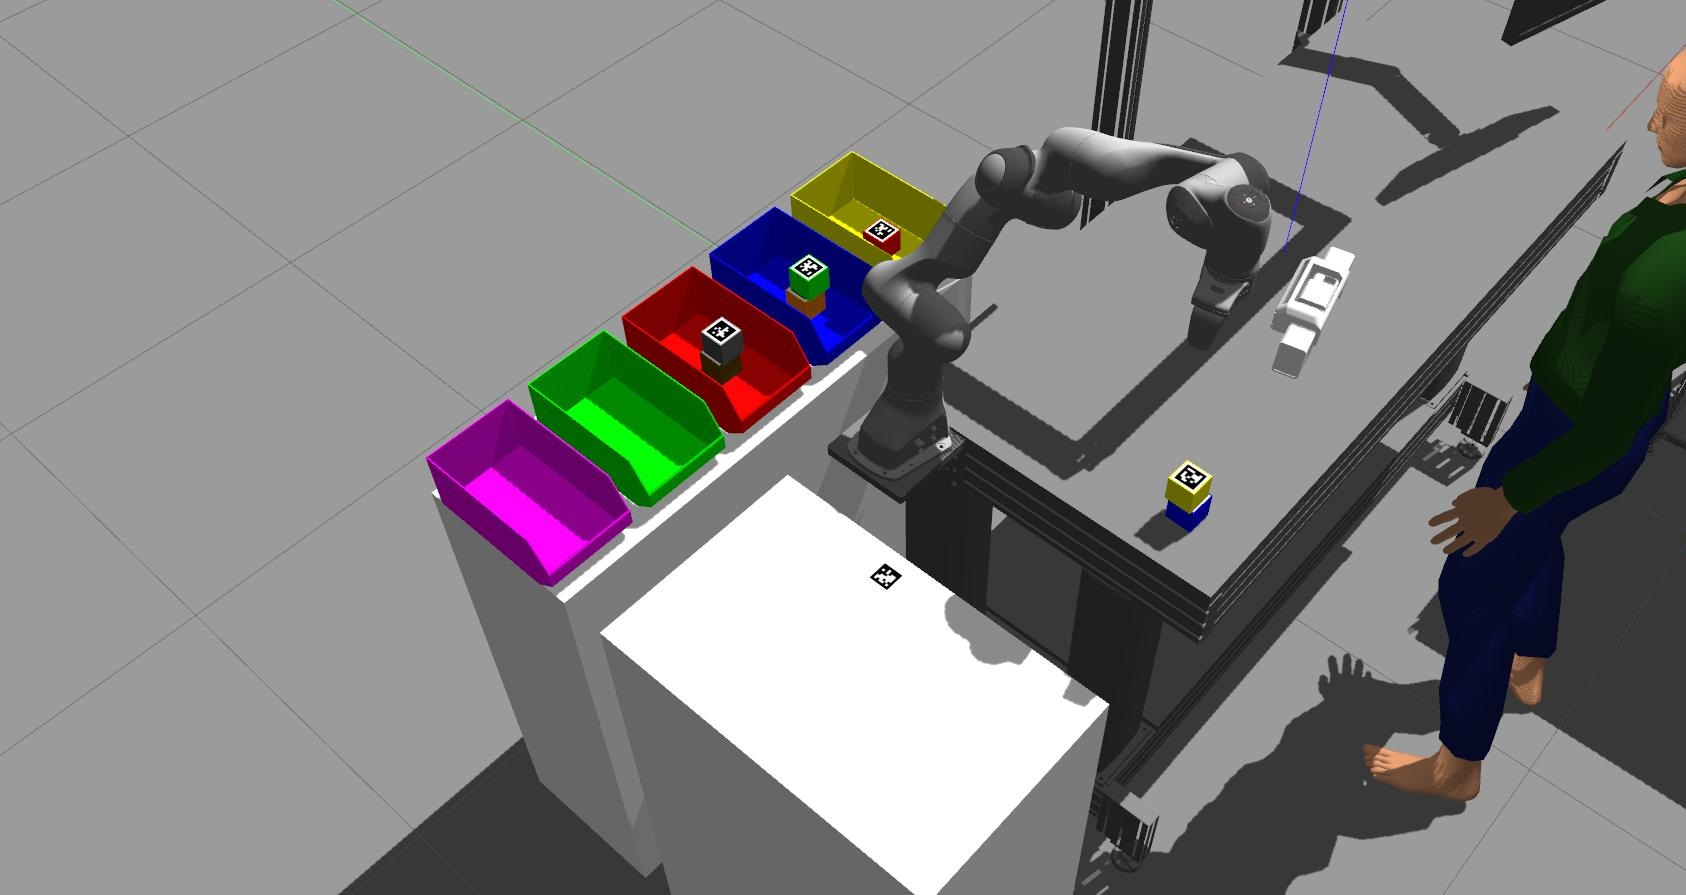
\includegraphics[width=0.6
\textwidth]{figures/Magistrale/ass_2}
\caption[BlockA Assembly Simulation]{
\label{fig:ass_2}}
\end{figure} 

\begin{figure} [h]
\centering
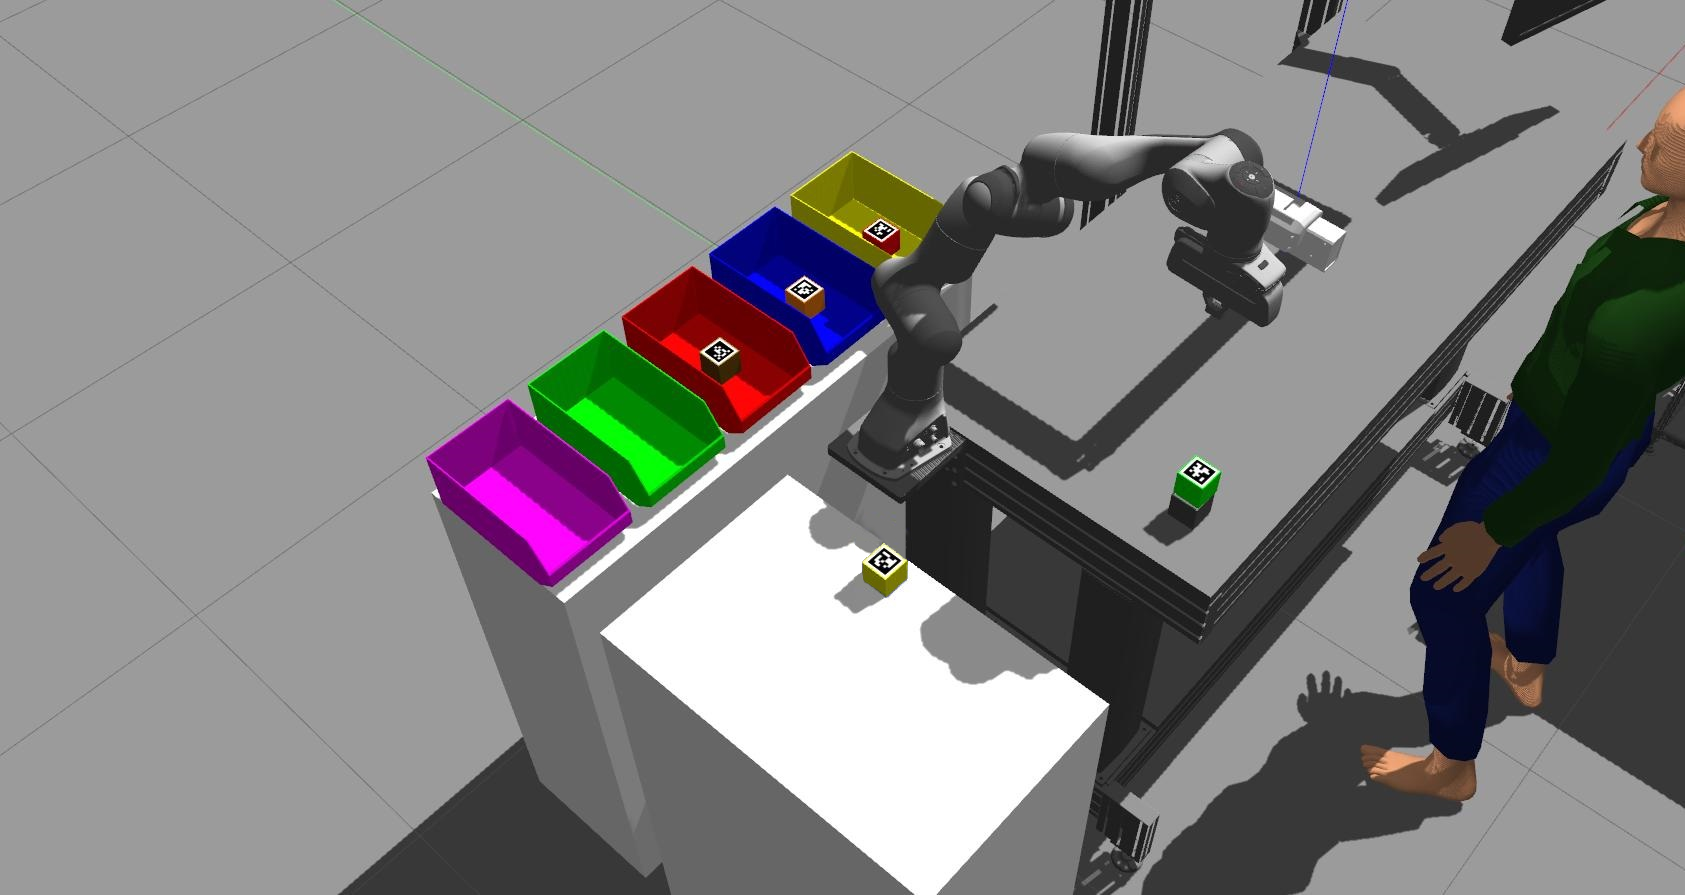
\includegraphics[width=0.6
\textwidth]{figures/Magistrale/ass_3}
\caption[First Part of BlockB Assembly Simulation]{
\label{fig:ass_3}}
\end{figure} 

\begin{figure} [h]
\centering
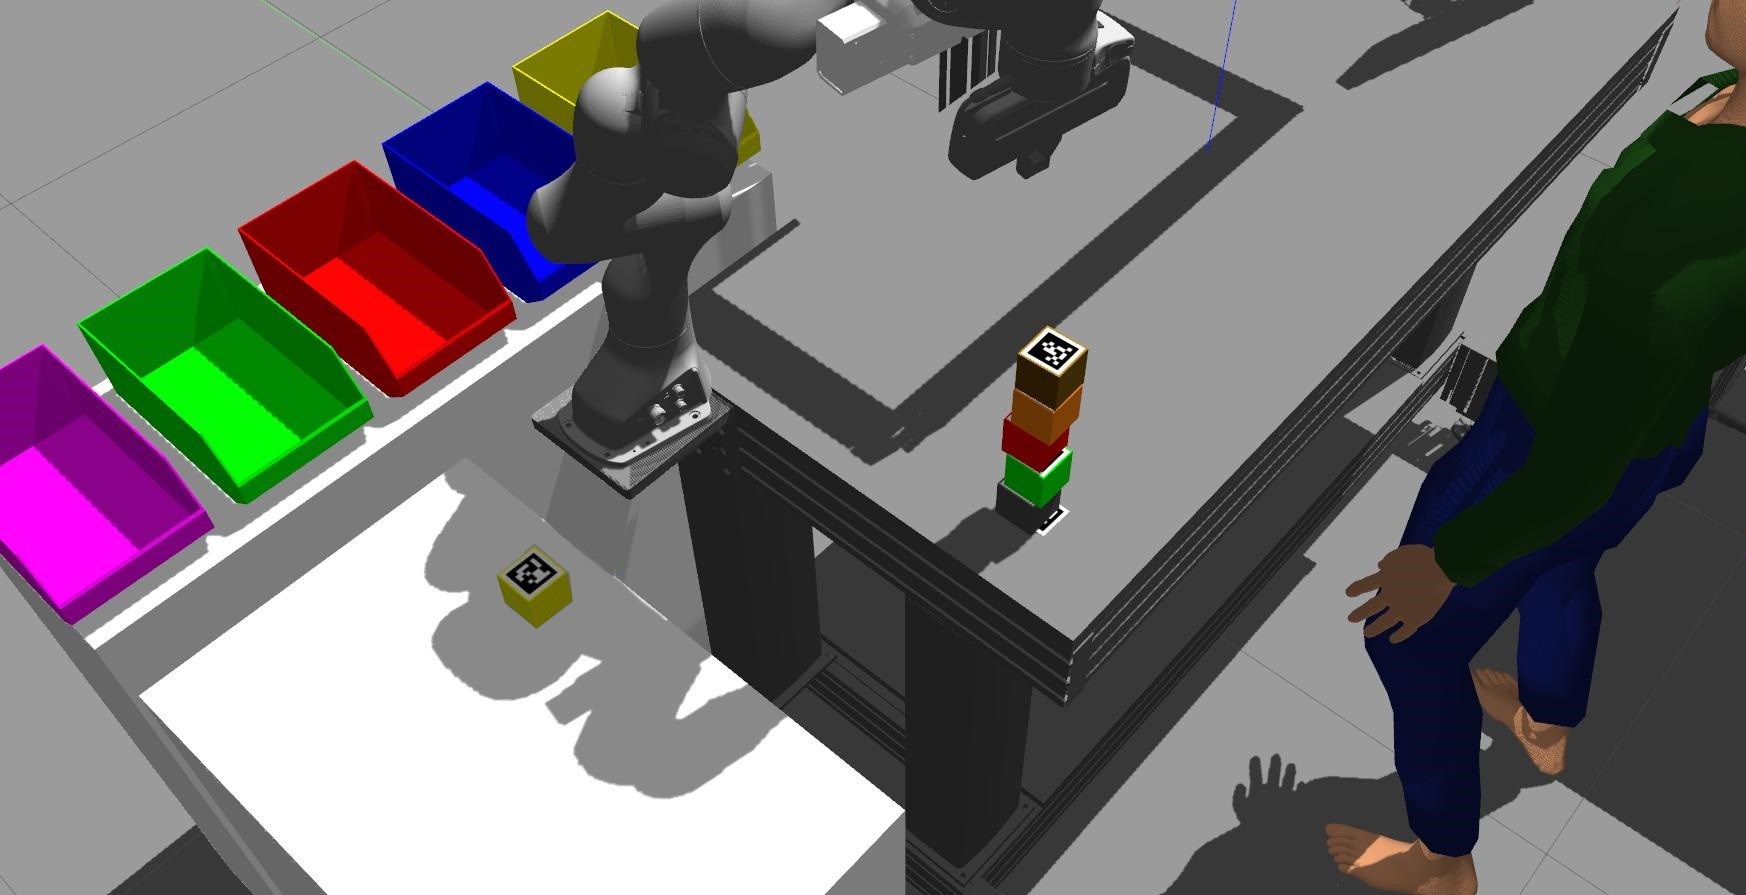
\includegraphics[width=0.6
\textwidth]{figures/Magistrale/ass_4}
\caption[Second Part of BlockB Assembly Simulation]{
\label{fig:ass_4}}
\end{figure} 


\section{Performance Considerations}\label{sec:perf_consid}

This project performs very simple tasks, since it only uses actions that pick up or place an object. 
It also uses a deprecated version to do NLP, which contains bugs and is limited in its logical understanding of sentences.
Consequently 
